\documentclass[11pt,a4paper]{article}

\usepackage{gastex}
\usepackage{etoolbox}
% \newcommand{\showLoesung}{2} %<---als Schalter
%\newcommand{\showInhalt}{1} %<---als Schalter

\usepackage{alltt,moreverb,amsmath,enumerate}
\usepackage[normalem]{ulem}
\usepackage[T1]{fontenc}
\usepackage{ae,aecompl} %helvet,mathptm
%\usepackage[left=15mm,right=15mm,top=20mm,bottom=20mm]{geometry}
\usepackage[margin=.5in]{geometry}
%\usepackage[latin1]{inputenc} % f�r Linux
\usepackage[utf8]{inputenc} % Umlaute etc. direkt schreiben (unter Windows)
\usepackage[german]{babel}
\usepackage[url]{oth-logoPNG}
%\usepackage{i2sym,i2ams}

\usepackage{tikz}
\usetikzlibrary{arrows,shapes,trees,positioning,automata,decorations.pathreplacing,decorations.pathmorphing}
\usepackage{tkz-graph}
\usepackage{color}

\usepackage{longtable}
\usepackage{tabularx}

%\usepackage{epic}
%\usepackage{eepic}
\usepackage{comment,ifthen}
\usepackage{../include/todo}

\usepackage[T1]{fontenc}
\usepackage{textcomp}

\usepackage{listings}                   % Listings in Core-Erlang und Maude
\usepackage{lstmisc}

\usepackage{epic}                       % Bildbefehle (picture)
%\usepackage{eepic}                      % erweiterte Bildbefehle

\usepackage{bbm}                        % Mengensymbole (N,C,R,B)
\usepackage{latexsym}                   % zusaetzliche Mathesymbole
\usepackage{amsmath}                    % Mathepaket von der AMS
\usepackage{amstext}
\usepackage{amsfonts}
\usepackage{stmaryrd}                   % zusaetzliche Mathesymbole
\usepackage{mathtools}
\usepackage{amsthm}
\usepackage{cancel}

\usepackage{hyperref}
\usepackage{url}                        % Zum Setzen von URLs in typewriter-face

\pagestyle{empty}

\let\epsilon=\varepsilon
\let\phi=\varphi

\frenchspacing

\setlength{\parindent}{0pt}
\setlength{\textwidth}{18.6cm}
\setlength{\textheight}{26.5cm}
\setlength{\hfuzz}{1mm}

%%% Read dates of assignments from file
\usepackage{xparse}
\ExplSyntaxOn
\ior_new:N \g_hringriin_file_stream

\NewDocumentCommand{\ReadFile}{mm}
 {
  \hringriin_read_file:nn { #1 } { #2 }
  \cs_new:Npn #1 ##1
   {
    \str_if_eq:nnTF { ##1 } { * }
      { \seq_count:c { g_hringriin_file_ \cs_to_str:N #1 _seq } }
      { \seq_item:cn { g_hringriin_file_ \cs_to_str:N #1 _seq } { ##1 } }
   }
 }

\cs_new_protected:Nn \hringriin_read_file:nn
 {
  \ior_open:Nn \g_hringriin_file_stream { #2 }
  \seq_gclear_new:c { g_hringriin_file_ \cs_to_str:N #1 _seq }
  \ior_map_inline:Nn \g_hringriin_file_stream
   {
    \seq_gput_right:cx 
     { g_hringriin_file_ \cs_to_str:N #1 _seq }
     { \tl_trim_spaces:n { ##1 } }
   }
  \ior_close:N \g_hringriin_file_stream
 }

\ExplSyntaxOff

\ReadFile{\uebungsabgabe}{../skel/UEBUNGSABGABE.def}

%%% Read subject info from file
\newcommand{\dozent}[1]{\def\DOZENT{#1}}
\newcommand{\tutoren}[1]{\def\TUTOREN{#1}}
\newcommand{\vorlesung}[1]{\def\VORLESUNG{#1}}
\newcommand{\semester}[1]{\def\SEMESTER{#1}}

\InputIfFileExists{../skel/VORLESUNG.def}{\providecommand{\TUTOREN}{}}%
{\typeout{***********}
 \typeout{Warnung: Kein File vorhanden, das die Vorlesung spezifiziert!}
 \typeout{Spezifikation muss daher im Text des Blattes oder ueber die
          Tastatur erfolgen.}
 \typeout{***********}}

\def\Uebung#1#2#3{
  \othLehrstuhlLogo[\DOZENT]
  \begin{center}
	{~\\[-2em]\Large\bf \VORLESUNG}\\[0.5em]
    \LARGE --~Tutorium #1 (Übung #2)~--\\[4mm]
  \
  \normalsize
  \textbf{#3}
    \rule{\textwidth}{0.1pt}\\[1cm]
  \end{center}
}

\def\Hinweis#1{
	{~\\[-3em]\bf Hinweis: }
	\begin{minipage}[t]{16.5cm}
	#1
	\end{minipage}\\[1em]
    \rule{\textwidth}{0.1pt}
}

\def\Tipps#1{
	{~\\[-3em]\bf Tipps: }
	\begin{minipage}[t]{16.5cm}
	#1
	\end{minipage}\\[1em]
    \rule{\textwidth}{0.1pt}
}
  
\def\MyHeader{
  \othLehrstuhlLogo[Prof.~Dr.~rer.~nat.~Carsten~Kern]%[Carsten~Kern,~Stefan~Rieger]
}

\newcommand{\sem}[1]{[\![#1\,]\!]}

\def\aufgabe#1#2{\subsection*{Aufgabe #1 (#2)}\par}
\def\endaufgabe{}

\newenvironment{loesung}{\subsection*{L\"osungsvorschlag:}}{}
\newenvironment{hinweis}{}{}
\ifthenelse{\isundefined{\showLoesung}}{\excludecomment{loesung}}{\pagestyle{plain}\excludecomment{hinweis}}

\newenvironment{tipps}{}{}
\ifthenelse{\isundefined{\showTipps}}{\excludecomment{tipps}}{\excludecomment{hinweis}}

\newenvironment{inhalt}{\subsection*{Kommentar:}}{}
\ifthenelse{\isundefined{\showInhalt}}{\excludecomment{inhalt}}{}

\long\def\Exercise#1#2{\begin{exercise}{#1}#2\end{exercise}}

\def\underbar#1{%
  \setbox0=\hbox{#1}%
  \dimen0=\dp0\relax%
  \dp0=0pt%
  \setbox0=\hbox{\underline{\box0}}%
  \dp0=\dimen0\relax%
  \box0%
  }

\makeatletter
\def\@makeunderbar[#1]#2{\expandafter\def\csname#1\endcsname{\underbar{#2}}}
\def\makeunderbar{\@ifnextchar[{\@makeunderbar}{\@makeunderbar[]}}
\makeatother

\def\T{\mathrm{T}}
\def\P{\mathrm{P}}
\def\CT{\mathrm{CT}}
\def\COp{\mathrm{COp}}

\makeunderbar{Comp}
\makeunderbar{Ops}
\makeunderbar{trans}
\makeunderbar[strans]{s-trans}
\makeunderbar[ntrans]{n-trans}
\makeunderbar{fix}

\def\labelenumi{\alph{enumi})}
\let\<=\langle
\let\>=\rangle

\parindent=0pt
\parskip=1ex

\definecolor{javared}{rgb}{0.6,0,0} % for strings
\definecolor{javagreen}{rgb}{0.25,0.5,0.35} % comments
\definecolor{javapurple}{rgb}{0.5,0,0.35} % keywords
\definecolor{javadocblue}{rgb}{0.25,0.35,0.75} % javadoc
 
\lstset{language=C++,
basicstyle=\ttfamily\footnotesize,
keywordstyle=\color{javapurple}\bf,
stringstyle=\color{javared},
commentstyle=\color{javagreen}\it\bf,
morecomment=[s][\color{javadocblue}]{/**}{*/},
numbers=left,
numberstyle=\tiny\color{gray},
stepnumber=1,
numbersep=10pt,
tabsize=3,
showspaces=false,
showstringspaces=false}

\usepackage{enumitem}
\usepackage{algpseudocode}
\usepackage{caption}
\usepackage{subcaption}
\usepackage{placeins}
\usepackage{multicol}
\usepackage{slashbox}
\usepackage{fancyvrb}
\usepackage{ulem}

\begin{document}
\thispagestyle{empty}
\DeclareRobustCommand{\ttfamily}{\fontencoding{T1}\fontfamily{lmtt}\selectfont}

\newcommand{\quotes}[1]{\glqq{}#1\grqq{}}

\Uebung{9}{10}{Simon Thelen}{9. Dezember 2021}  % FIXME: Blattnummer, Datum, Zeit

%%%%%%%%%%%%%%%%%%%%%%%%%%%%%%%%%%%%%%%%%%%%%%%%%%%%%%%%%%%%%%%%%%%%%%

\ifcsdef{showLoesung}{
\textbf{Bitte beachten Sie:} Die Lösungen können trotz sorgfältiger Prüfung Fehler enthalten.
Bei Fragen oder Unklarheiten kontaktieren Sie bitte den Tutor oder Dozenten in Tutorien, Übungen oder nach Vorlesungen.
}{}


\begin{aufgabe}{1}{Hashing}
    \begin{enumerate}
        \item Gegeben sei eine Hashtabelle mit $100$ Plätzen, die Hashing mit Verkettung verwendet.
        Es werden $150$ Werte mithilfe einer gleichmäßig verteilenden Hashfunktion eingefügt.
        Berechnen Sie die Wahrscheinlichkeit, dass ein bestimmter Platz der Tabelle nach dem Einfügen genau ein Element enthält.
        \item Sei $X$ die Anzahl der Plätze der obigen Tabelle, die nach Einfügen von 150 Werten genau ein Element enthalten.
        Berechnen Sie $E[X]$ mithilfe des \quotes{5-Punkte-Plans} und des Ergebnisses der vorherigen Teilaufgabe~(Wenn Sie die vorherige Aufgabe nicht lösen konnten, verwenden Sie $P(\text{ein Element}) = \frac{1}{3}$).
    \end{enumerate}
\end{aufgabe}

\begin{loesung}
    \begin{enumerate}
        \item Betrachten wir zunächst den Fall, dass der erste der 150 Werte in den gewünschten Platz einsortiert wird und alle weiteren 149 Elemente in einen anderen.
        Die Wahrscheinlichkeit, dass ein Wert in den rich\-ti\-gen Platz einsortiert wird, ist $\frac{1}{100}$, die Wahrscheinlichkeit, dass es ein anderer Platz ist, $\frac{99}{100}$.
        Da alle Werte unabhängig voneinander einsortiert werden, können die Wahrscheinlichkeiten für alle Werte einfach multipliziert werden.
        Die Wahrscheinlichkeit dafür, dass der erste der 150 Werte in den gewünschten Platz einsortiert wird und alle weiteren 149 Elemente in einen anderen, beträgt also $\frac{1}{100}\cdot \left(\frac{99}{100}\right)^{149}$.

        Jetzt muss der eine Wert, der in den gewünschten Platz einsortiert wird, aber nicht unbedingt der erste sein, sondern es kann jeder der 150 Werte sein.
        Da sich die Wahrscheinlichkeiten der einzelnen Plätze jedoch für die anderen Werte nicht ändern, gilt die obige Wahrscheinlichkeit für alle 150 Werte.

        Es muss nur noch die Wahrscheinlichkeit berechnet werden, dass mindestens eines der obigen 150 Ereignisse eintritt.
        Allerdings sind alle Ereignisse disjunkt (es kann maximal eines eintreten).
        Daher reicht es, alle 150 Wahrscheinlichkeiten aufzusummieren.
        Das finale Ergebnis ist also $150 \cdot \frac{1}{100}\cdot \left(\frac{99}{100}\right)^{149} \approx 33.6\%$. 

        \item
        \begin{description}
            \item[Schritt 1: Definiere eine geeignete Zählvariable.]
            Wir wollen die Plätze der Tabelle zählen, die genau einen Wert enthalten.
            Daher definieren wir die Zählvariable wie folgt:
            \begin{equation*}
                X_i = \begin{cases}
                    1 & \text{Der $i$-te Platz enthält genau einen Wert} \\
                    0 & \text{sonst}
                \end{cases}
            \end{equation*}
            \item[Schritt 2: Bestimme die Wahrscheinlichkeit, dass $X_i = 1$.]
            Die Situation, dass $X_i = 1$ entspricht genau der betrachteten Situation aus der vorherigen Teilaufgabe.
            Also: $P(X_i = 1) = 150 \cdot \frac{1}{100}\cdot \left(\frac{99}{100}\right)^{149} \approx 33.6\%$.
            \item[Schritt 3: Bestimme den Erwartungswert von $X_i$.]
            \begin{equation*}
                E[X_i] = 1 \cdot P(X_i = 1) + 0 \cdot P(X_i = 0) = P(X_i = 1) + 0 \approx 33.6\%
            \end{equation*}
            \item[Schritt 4: Definiere neue Zählvariable.]
            Wir definieren $X = \sum\limits_{i = 1}^{100} X_i$
            \item[Schritt 5: Bestimme den Erwartungswert von $X$.]
            \begin{equation*}
                E[X] = E\left[ \sum\limits_{i = 1}^{100} X_i \right]
                \overset{\text{Linearität von $E$}}{=} \sum\limits_{i = 1}^{100} E[X_i]
                \overset{\text{Schritt 3}}{\approx} \sum\limits_{i = 1}^{100} 33.6\% = 100 \cdot 33.6\% = 33.6
            \end{equation*}
        \end{description}
        
    \end{enumerate}
\end{loesung}

\begin{aufgabe}{2}{Skip-Listen}
    \begin{enumerate}[label=\alph*)]
        \item Fügen Sie folgende Werte in eine leere Skip-Liste ein:
        5 (mit Höhe 2), 7 (1), 3 (3), 8 (2), 1 (1), 2 (2), 4 (1).
        Löschen Sie anschließend folgende Werte: 7, 5, 3.
        % \item Führe folgende Operationen sukzessiv auf einer leeren Skip-Liste aus (\texttt{Insert($v$, $h$)} fügt den Wert $v$ mit Höhe $h$ in die Liste ein): TODO\ldots.
        Geben Sie bei jeder Operation an, auf welche Knoten lesend und schreibend zugegriffen wird.
        % 5, 2
        % 7, 1
        % 2, 3
        % 8, 2
        % 0, 1
        % 1, 2
        % 4, 1
        \item Zeigen Sie mittels des \quotes{5-Punkte-Plans}, dass die erwartete Höhe eines Wertes einer Skip-Liste 2 beträgt, indem Sie die folgenden Zählvariablen verwenden:
        \begin{equation*}
            X_i = \begin{cases}
                1 & \text{der Wert hat mindestens Höhe $i$} \\
                0 & \text{sonst}
            \end{cases}
        \end{equation*}
        \item\label{skip} 
        Erweitern Sie die Skip-Listen-Datenstruktur, sodass zusätzlich zu jedem Zeiger gespeichert wird, wie viele Werte übersprungen werden, wenn man über diesen Zeiger zum entsprechenden Wert springt.
        Beschreiben Sie kurz, wie die Einfüge- und Lösch-Operationen für diese Erweiterung angepasst werden müssen, ohne das asymptotische Laufzeitverhalten zu verändern.

        \item 
        Implementieren Sie auf Basis der Erweiterung aus Teilaufgabe \ref*{skip} die Operation \textsc{KthSmallestValue} in Pseudocode oder einer Programmiersprache Ihrer Wahl mit durchschnittlicher Laufzeit $O(\log n)$, welche Ihnen den $k$-kleinsten Wert der Liste liefert.
    \end{enumerate}
\end{aufgabe}

\begin{loesung}
    \begin{enumerate}
        \item Im folgenden sind Knoten, auf die lesend zugegriffen wird, blau, Knoten, auf die schreibend zugegriffen wird, rot, und Knoten, auf die sowohl lesend als auch schreibend zugegriffen wird, gelb markiert.
        \begin{figure}[h!]
            \centering
            \begin{subfigure}[b]{0.3\textwidth}
                \centering
                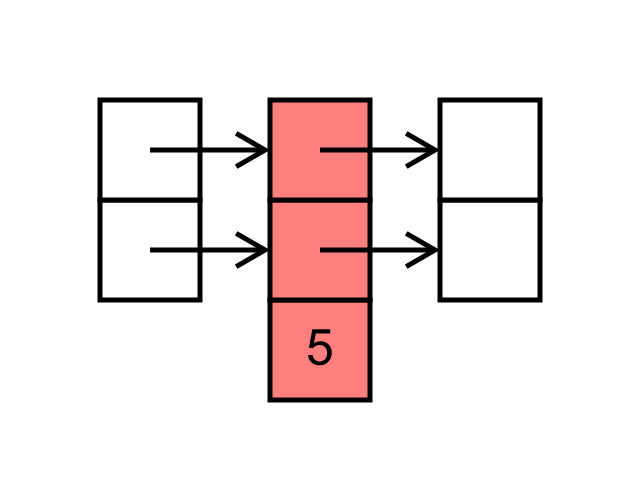
\includegraphics[scale=0.15]{img/2a/1}
            \end{subfigure}
            \begin{subfigure}[b]{0.3\textwidth}
                \centering
                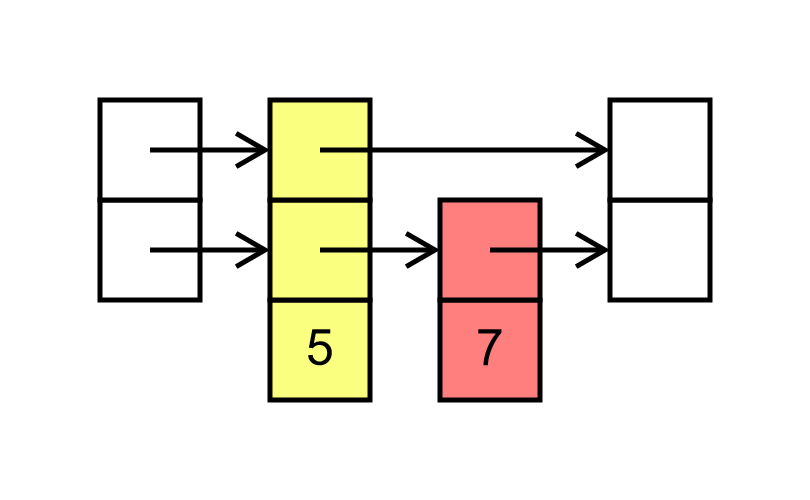
\includegraphics[scale=0.15]{img/2a/2}
            \end{subfigure}
            \begin{subfigure}[b]{0.3\textwidth}
                \centering
                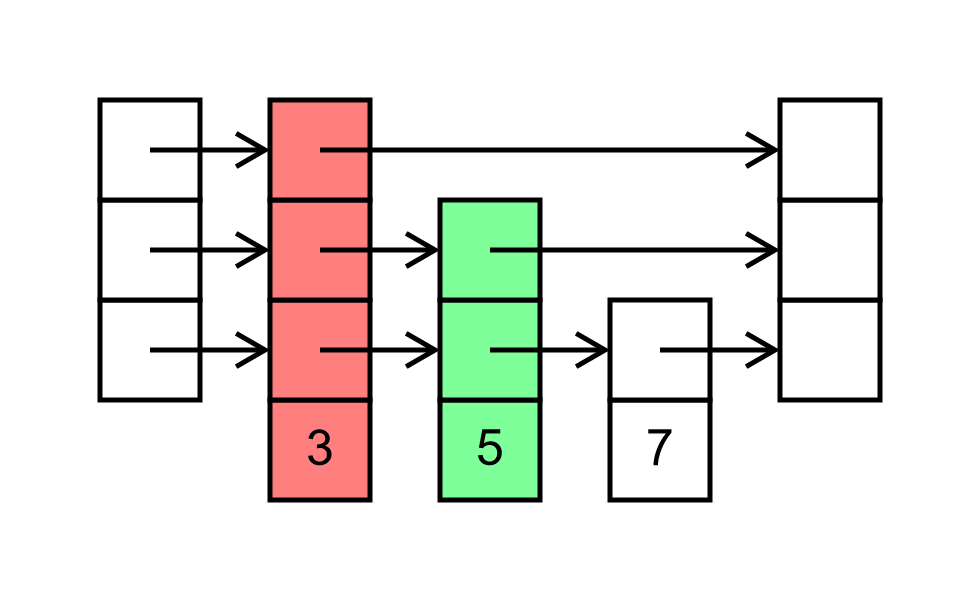
\includegraphics[scale=0.15]{img/2a/3}
            \end{subfigure}
        \end{figure}
        \begin{figure}[h!]
            \centering
            \begin{subfigure}[b]{0.45\textwidth}
                \centering
                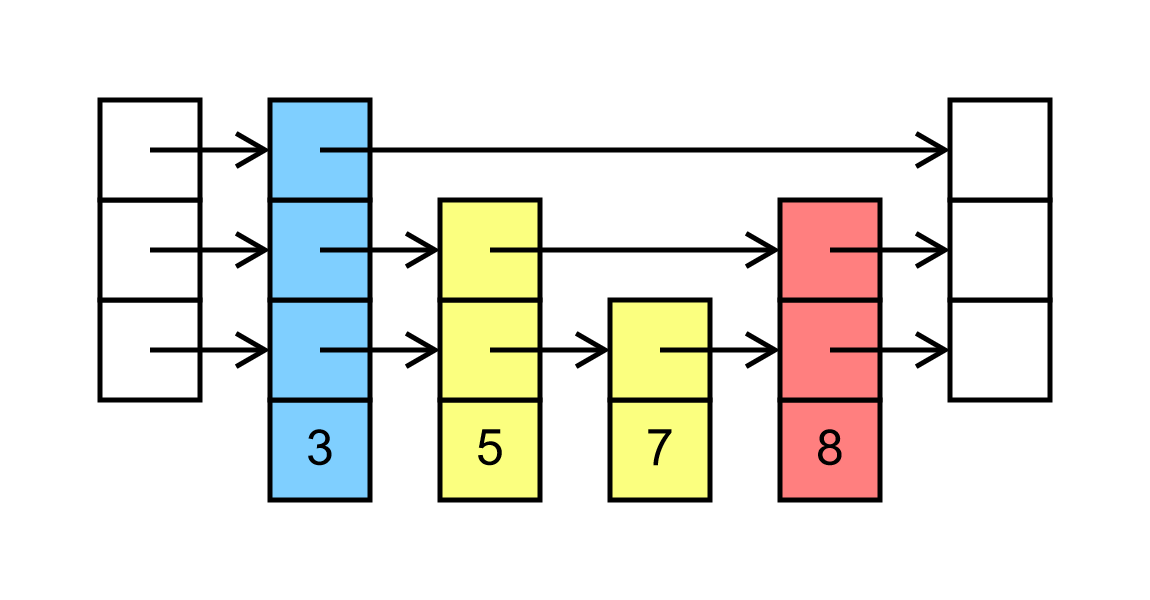
\includegraphics[scale=0.15]{img/2a/4}
            \end{subfigure}
            \begin{subfigure}[b]{0.45\textwidth}
                \centering
                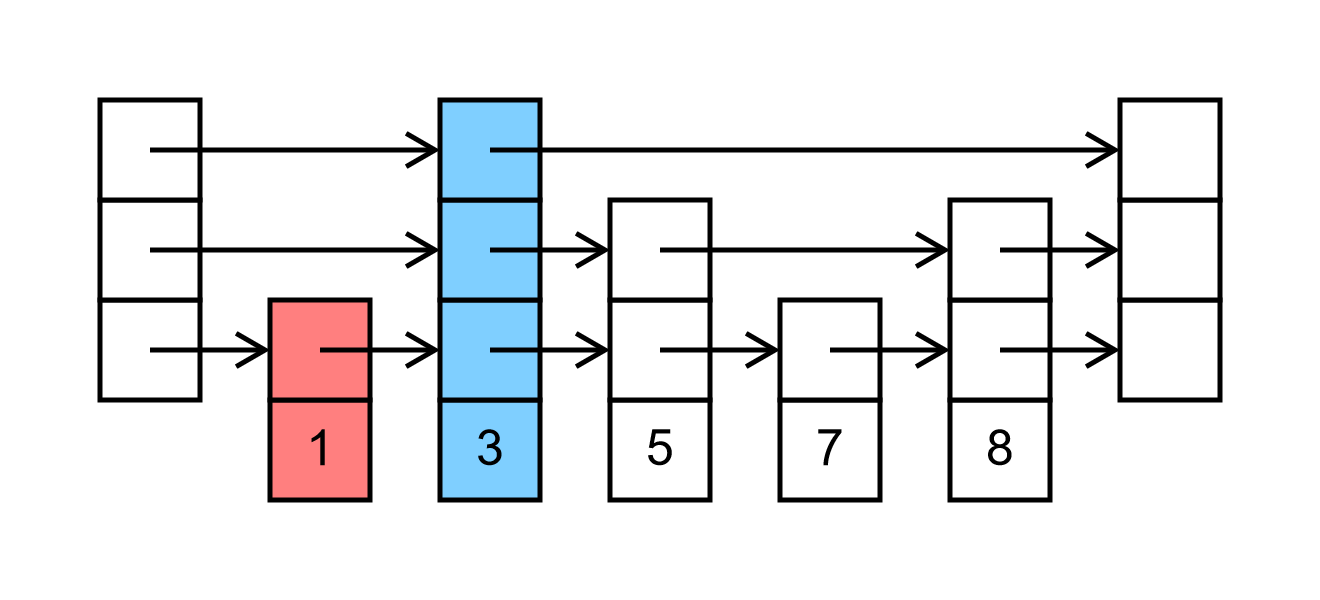
\includegraphics[scale=0.15]{img/2a/5}
            \end{subfigure}
        \end{figure}
        \begin{figure}[h!]
            \centering
            \begin{subfigure}[b]{0.45\textwidth}
                \centering
                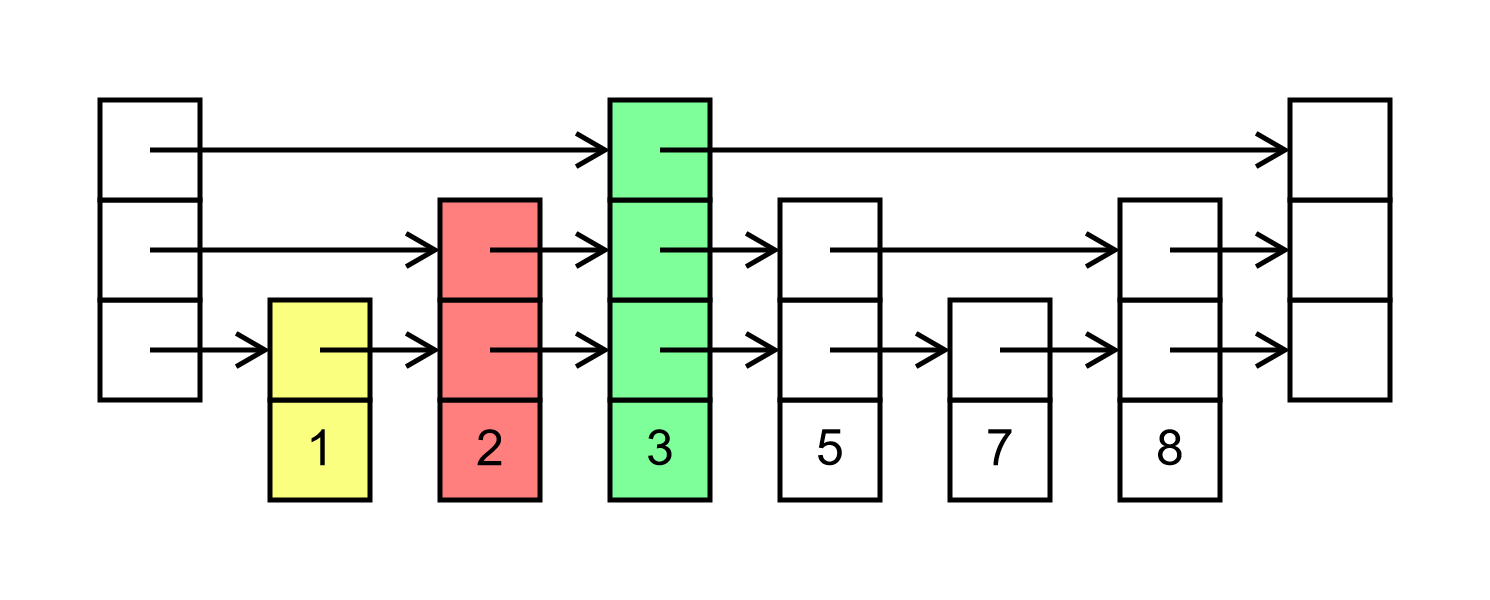
\includegraphics[scale=0.14]{img/2a/6}
            \end{subfigure}
            \begin{subfigure}[b]{0.45\textwidth}
                \centering
                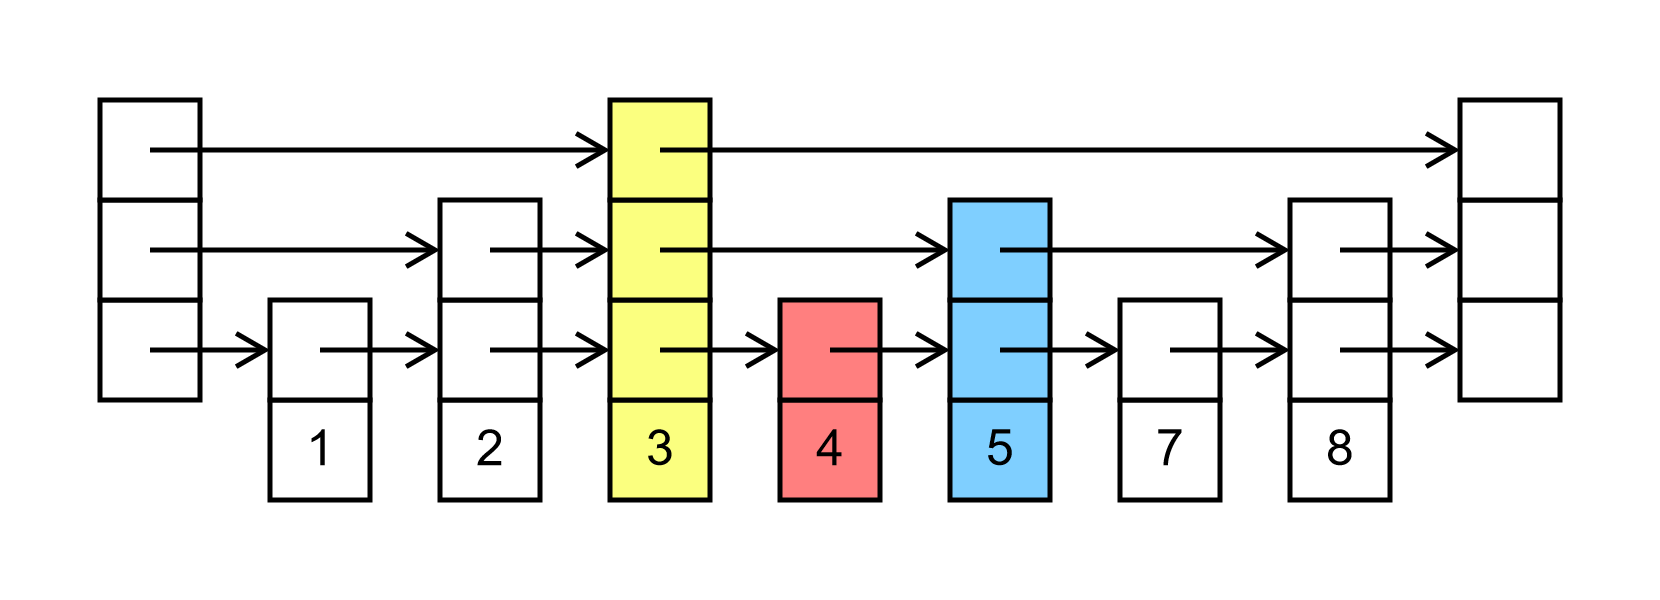
\includegraphics[scale=0.14]{img/2a/7}
            \end{subfigure}
        \end{figure}
        \begin{figure}[h!]
            \centering
            \begin{subfigure}[b]{0.45\textwidth}
                \centering
                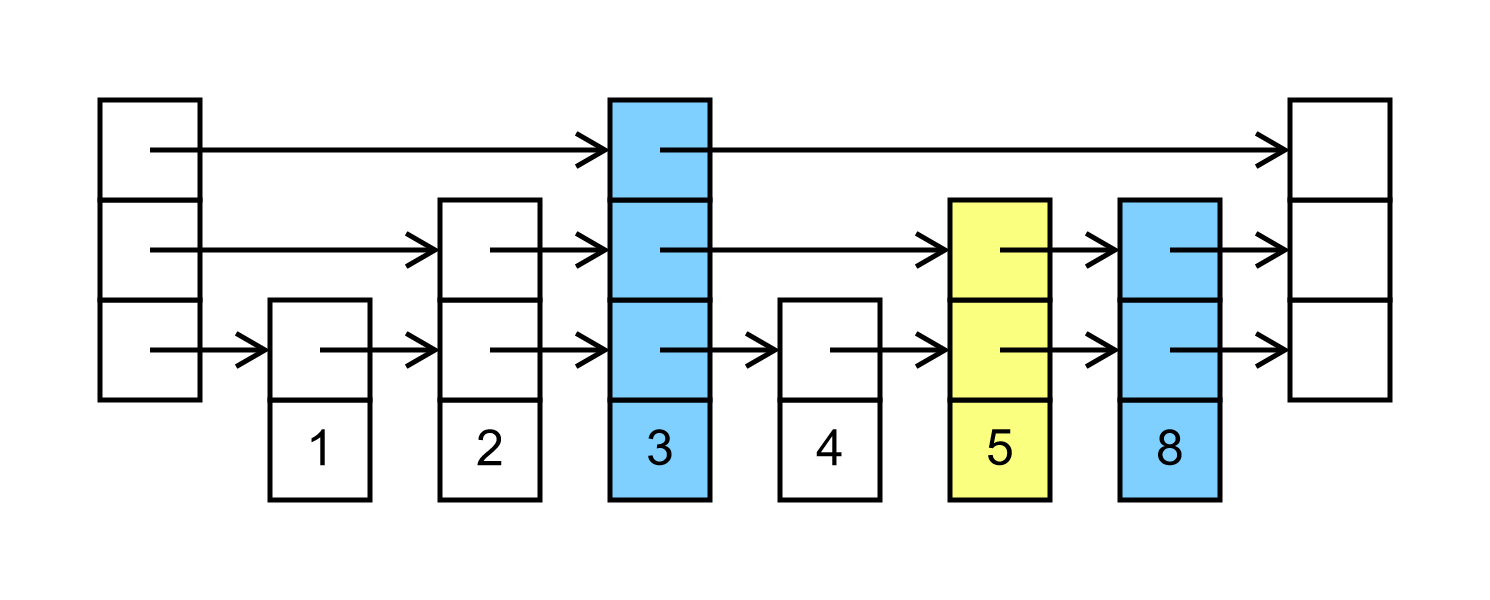
\includegraphics[scale=0.15]{img/2a/8}
            \end{subfigure}
            \begin{subfigure}[b]{0.45\textwidth}
                \centering
                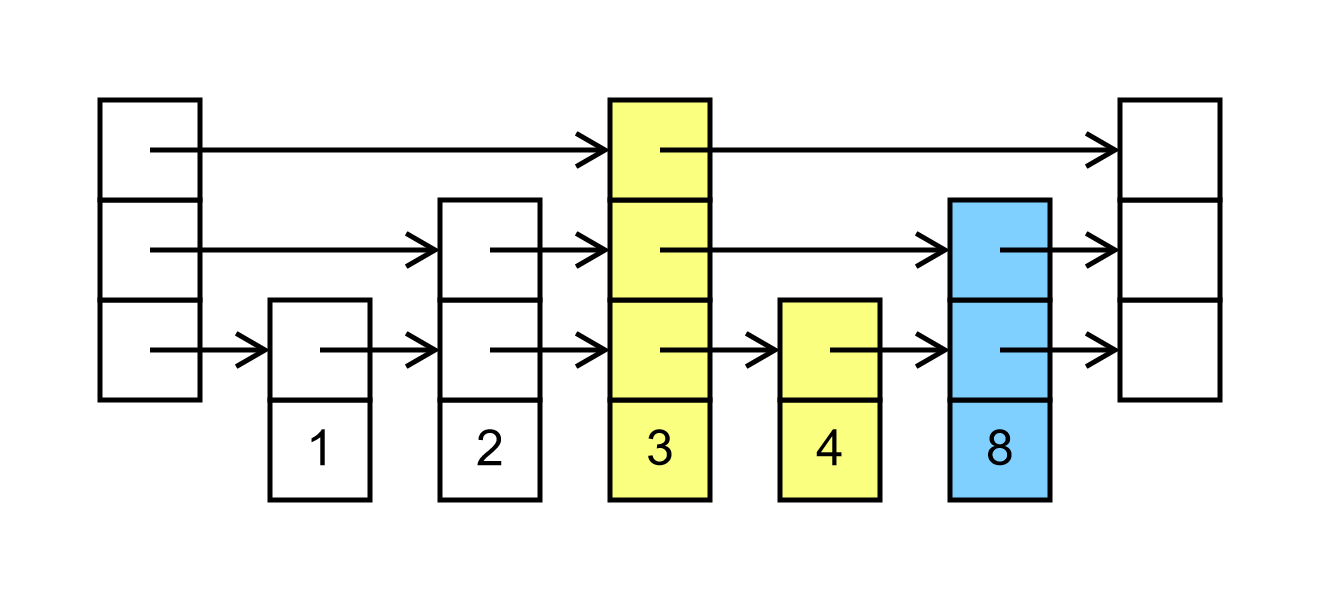
\includegraphics[scale=0.15]{img/2a/9}
            \end{subfigure}
        \end{figure}
        \begin{figure}[h!]
            \centering
            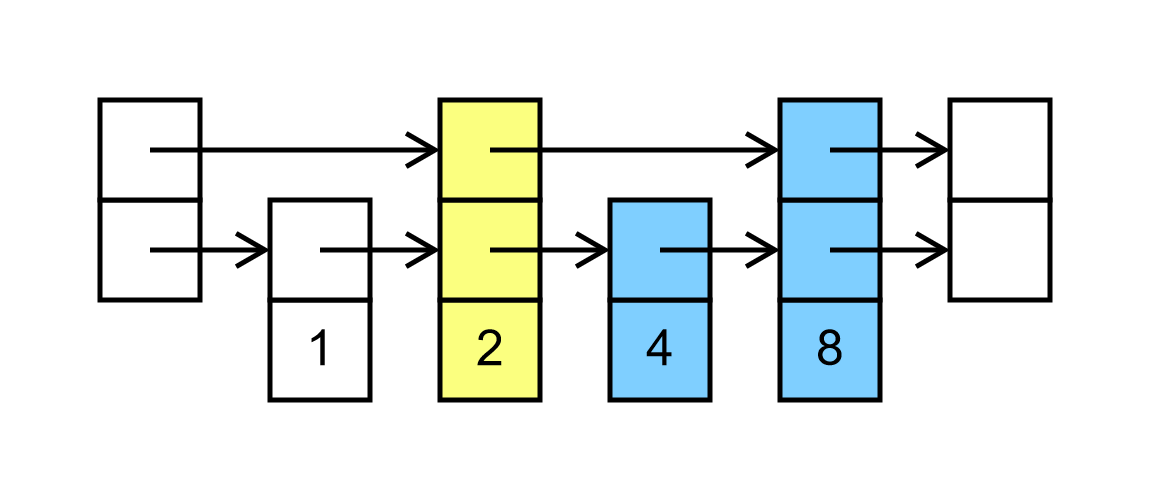
\includegraphics[scale=0.15]{img/2a/10}
        \end{figure}
        \FloatBarrier
        \item
        \begin{description}
            \item[Schritt 1: Definiere eine geeignete Zählvariable.]
            Wir verwenden die Variable aus der Aufgabenstellung:
            \begin{equation*}
                X_i = \begin{cases}
                    1 & \text{der Wert hat mindestens Höhe $i$} \\
                    0 & \text{sonst}
                \end{cases}
            \end{equation*}
            \item[Schritt 2: Bestimme die Wahrscheinlichkeit, dass $X_i = 1$.]
            Die Wahrscheinlichkeit, dass die Höhe mindestens $i$ beträgt, entspricht 1 minus der Gegenwahrscheinlichkeit, nämlich dass die Höhe maximal $i - 1$ ist ($P(\text{Höhe genau $h$}) = (1 / 2)^h$).
            Es gilt also:
            \begin{align*}
                P(X_i = 1) &= P(\text{Höhe min. $i$})
                = 1 - \sum\limits_{h = 1}^{i - 1} \left(\frac{1}{2}\right)^h \\
                &= 1 - \left(\sum\limits_{h = 0}^{i - 1} \left(\frac{1}{2}\right)^h\right) + \underbrace{\left(\frac{1}{2}\right)^0}_{= 1}
                \overset{\text{Geom. Reihe}}{=} 2 - \frac{\left(\frac{1}{2}\right)^i - 1}{\frac{1}{2} - 1} \\
                &= 2 - (-2) \cdot \left(\left(\frac{1}{2}\right)^i - 1\right)
                = 2 + 2 \cdot \left(\frac{1}{2}\right)^i - 2
                = 2 \cdot \left(\frac{1}{2}\right)^i \\
                &= \left(\frac{1}{2}\right)^{-1} \cdot \left(\frac{1}{2}\right)^i
                = \left(\frac{1}{2}\right)^{i - 1}
            \end{align*}
            \item[Schritt 3: Bestimme den Erwartungswert von $X_i$.]
            \begin{equation*}
                E[X_i] = 1 \cdot P(X_i = 1) + 0 \cdot P(X_i = 0) = P(X_i = 1) + 0 = \left(\frac{1}{2}\right)^{i - 1}
            \end{equation*}
            \item[Schritt 4: Definiere neue Zählvariable.]
            Wir definieren $X = \sum\limits_{i = 1}^{\infty} X_i$
            \item[Schritt 5: Bestimme den Erwartungswert von $X$.]
            \begin{align*}
                E[X] &= E\left[ \sum\limits_{i = 1}^{\infty} X_i \right]
                \overset{\text{Linearität von $E$}}{=} \sum\limits_{i = 1}^{\infty} E[X_i]
                \overset{\text{Schritt 3}}{=} \sum\limits_{i = 1}^{\infty} \left(\frac{1}{2}\right)^{i - 1} \\
                &= \sum\limits_{i = 0}^{\infty} \left(\frac{1}{2}\right)^i
                \overset{\text{unendl. Geom. Reihe}}{=} 2
            \end{align*}
        \end{description}
        \item
        \begin{description}
            \item[Einfügen] 
            Beim Einfügen wird ja entlang der Zeiger in der Skip-Liste gesprungen, um die Position zu erreichen, an die der Wert eingefügt werden soll.
            Durch die zusätzlichen Werte, die beschreiben, wie viele Werte bei jedem Springen übersprungen werden, kann man leicht feststellen, an welche Position der neue Wert eingefügt wird, indem man die Werte für alle Zeiger, die fürs Einfügen durchlaufen werden, aufsummiert und dazu noch alle Knoten mitzählt, die man fürs Einfügen passiert.
            Nach dem Einfügen geht man erneut den Weg zum eingefügten Knoten.
            Die Werte zu allen Zeigern, die den eingefügten Knoten überspringen, erhöht man um 1.
            Für jeden Zeiger, den man zuvor beim Einfügen aktualisiert hat, kennt man durch das oben beschriebene Verfahren die Position des zugehörigen Knotens.
            Aus dem ursprünglichen Überspring-Wert des Zeigers, dessen Position und der Position des eingefügten Wertes kann man die beiden neuen Werte leicht berechnen.
            Dabei geht man wie in folgendem Beispiel vor:
            Ein Zeiger des Knotens an Position 3 übersprang vor dem Einfügen 10 Werte und zeigte somit auf Position 14 ($=3 + 10 + 1$).
            Jetzt wurde ein neuer Wert an Position 7 eingefügt und der Zeiger zeigt auf diesen eingefügten Wert.
            Damit überspringt der Zeiger nun $7 - 3 - 1 = 4$ Werte.
            Der neue Wert (an Position 7) zeigt ja jetzt auf Position 14 und überspringt dadurch $14 - 7 - 1 = 6$ Werte.
            
            Man muss den Pfad zum eingefügten Wert also nur zweimal durchlaufen.
            An jeder Position des Pfads wird weiterhin nur konstante Laufzeit benötigt.
            Das asymptotische Laufzeitverhalten ändert sich also nicht. 
            \item[Löschen]
            Zunächst sucht man den zu gewünschten Wert in der Liste, ohne ihn tatsächlich zu löschen.
            Dabei bestimmt man, wie oben beschrieben dessen Position.
            Wenn man den Pfad zum Knoten nun ein weiteres Mal durchläuft, um ihn zu löschen, geht man ähnlich wie beim Einfügen vor:
            Werte von Zeigern, die den zu löschenden Knoten überspringen, verringert man um 1.
            Bei Zeigern, die auf den zu löschenden Wert zeigen, geht man wie im folgenden Beispiel vor.
            Angenommen, ein Knoten $a$ zeigt auf den zu löschenden Knoten $b$ und überspringt dabei 4 Werte.
            Der Zeiger des zu löschenden Knotens auf gleicher Höhe zeigt auf $c$ und überspringt dabei 6 Werte.
            Wird dann $b$ gelöscht, zeigt nun $a$ auf $c$.
            Dabei werden $4 + 6 = 10$ Werte übersprungen.

            Nach der gleichen Argumentation wie schon beim Einfügen ändert sich bei dieser Anpassung das Laufzeitverhalten nicht.
        \end{description}
        \item Wir gehen für die Lösung von folgender Skip-List-Implementierung aus:
        \begin{lstlisting}[language=c++]
class Node {
    public:
    int value;
    int height;
    Node *next[MAX_HEIGHT];
    int skip[MAX_HEIGHT];
};
class SkipList {
    public:
    int height;
    Node *nodes[MAX_HEIGHT];
    int skip[MAX_HEIGHT];
};
        \end{lstlisting}
        Die Idee ist simpel:
        Wir traversieren genau so über die Liste, wie wir das beim normalen Suchen auch tun würden.
        Jedoch hängt die Entscheidung, ob wir einen Zeiger entlang zum nächsten Knoten gehen oder eine Ebene nach unten, nicht davon ab, ob der Wert des nächsten Knotens größer ist als der gesuchte, sondern ob dessen Position größer ist als die gesuchte.
        Die Position errechnet sich über die Position des aktuellen Knotens plus der Anzahl der Knoten, die übersprungen werden, plus 1 (der Zielknoten muss auch mitgezählt werden).
        Sobald die gewünschte Position erreicht wurde, kann der entsprechende Wert zurückgegebenen werden.
        \begin{lstlisting}[language=c++]
int kthSmallestValue(SkipList *list, int k) {
    int i;
    int pos = 0;
    Node *node = nullptr;
    for (i = list->height - 1; i >= 0; i--) {
        if (list->skip[i] < k) {
            node = list->nodes[i];
            pos = list->skip[i] + 1;
            break;
        }
    }
    while (pos != k) {
        if (node->next[i] == nullptr) {
            // index out of bounds
            return -1;
        }
        for (; i >= 0; i--) {
            if (pos + list->skip[i] < k) {
                node = node->next[i];
                pos += node->skip[i] + 1;
                break;
            }
        }
    }
    return node->value;
}
        \end{lstlisting}
    \end{enumerate}
\end{loesung}

\begin{aufgabe}{3}{Textsuche}
    \begin{enumerate}[label=\alph*)]
        \item Betrachten Sie das Muster \texttt{BEENDEN}.
        Wie ist die \texttt{shift}-Funktion für dieses Muster mit $\Sigma = \{A, B, \ldots, Z\}$ bei Verwendung der Bad-Character-Strategie definiert?
        Sie dürfen alle Zeichen, die nicht im Muster enthalten sind, zusammenfassen.
        \item Betrachten Sie die Muster \texttt{KENNEN}, \texttt{NENNEN} und \texttt{NONNEN}.
        Geben Sie für beide Muster und für jede Position an, um viel viele Zeichen das jeweilige Muster gemäß der Good-Suffix-Strategie verschoben werden darf, wenn es an dieser Position zu einer Nichtübereinstimmung kommt.
        \item Suchen Sie das Muster \texttt{CTGCAGC} in der Zeichenkette \texttt{TATGAAAGCTGCCGCGCTGCAGCCGC} mittels Naiver Suche und mithilfe des Boyer-Moore-Algorithmus inklusive bad-character und good-suffix.
        Wie viele Vergleiche benötigen Sie jeweils?
        \item 
        Suchen Sie das Muster \texttt{LEBEN} im Text \texttt{DAS ENDE EINES LEBENS} mittels Boyer-Moore.
        Verwenden Sie dafür einmal die Bad-Character-, einmal die Horspool- und einmal die Sunday-Heuristik.
        Kombinieren Sie schließlich alle drei Heuristiken.
        Wie viele Vergleiche benötigen Sie jeweils?
        % DAS ENDE DES LEBENS
        % LEBEN
        %  LEBEN
        %     LEBEN
        %          LEBEN
        %              LEBEN
        % DAS ENDE DES LEBENS
        % LEBEN
        %  LEBEN
        %       LEBEN
        %        LEBEN
        %             LEBEN
        %              LEBEN
        % DAS ENDE DES LEBENS
        % LEBEN
        %  LEBEN
        %        LEBEN
        %              LEBEN
        % DAS ENDE EINES LEBENS
        % LEBEN
        %  LEBEN
        %     LEBEN
        %          LEBEN
        %               LEBEN
        %                LEBEN
        % DAS ENDE EINES LEBENS
        % LEBEN
        %  LEBEN
        %       LEBEN
        %            LEBEN
        %                LEBEN
        % DAS ENDE EINES LEBENS
        % LEBEN
        %  LEBEN
        %        LEBEN
        %          LEBEN
        %                LEBEN
        % DAS ENDE EINES LEBENS
        % LEBEN
        %  LEBEN
        %        LEBEN
        %             LEBEN
        %                LEBEN
        \item Geben Sie ein Beispiel für eine Eingabe (Text und Muster) an, bei der der Boyer-Moore-Algorithmus unter Verwendung der Bad-Character-Strategie deutlich mehr Vergleiche benötigt als die naive Suche.
        Verallgemeinern Sie anschließend Ihre Beispiel-Eingabe, indem eine Regel für beliebig lange \quotes{bösartige} Eingaben angeben und bestimmen Sie die asymptotischen Worst-Case-Laufzeiten, die \texttt{NaiveSearch} und Boyer-Moore auf diesen Eingaben benötigen (abhängig von $n$ und $m$).
        % \item In der Boyer-Moore-Implementierung aus den Vorlesungsunterlagen wird, sobald das Muster gefunden wurde, das Muster nur um 1 nach rechts geschoben, bevor weiter gesucht wird.
        % Machen Sie einen Vorschlag zu einer möglichen Optimierung, indem Sie Ideen aus der Vorlesung verwenden.

        \item Erstellen Sie einen deterministischen, endlichen Automat über dem Alphabet $\Sigma = \{\text{\texttt{A}}, \text{\texttt{B}}, \text{\texttt{C}}\}$ mit 7 Zuständen, welcher Vorkommen der des Musters \texttt{ABCABA} in einer Zeichenkette erkennt.
        Der Automat soll die zu durchsuchende Zeichenkette Zeichen für Zeichen einlesen und mit jedem gelesenden Zeichen gemäß seiner Transitionen in einen anderen Zustand wechseln.
        Jedes Mal, wenn ein ausgewiesener Endzustand erreicht wird, wurde ein weiteres Vorkommen des Musters gefunden.
        Beschreiben Sie den Automaten eindeutig, zum Beispiel, indem Sie dessen Transitionsgraph angeben.
        \item Betrachten Sie folgenden Suchalgorithmus:
        Sämtliche Teilstrings des zu durchsuchenden Texts werden in einer Hashtabelle abgespeichert (bei \quotes{abc} also z.B. \quotes{a}, \quotes{b}, \quotes{c}, \quotes{bc}, \quotes{ab}, \quotes{abc}).
        Wenn nun ein Muster im Text gesucht werden soll, muss nur überprüft werden, ob das Muster in der Hashtabelle liegt.
        Geben Sie folgende Funktionen in $O$-Notation an, jeweils abhängig von der Länge des Textes $n$ und der Länge des Musters $m$:
        \begin{enumerate}[label=\roman*)]
            \item die durchschnittliche Laufzeit zum Erstellen der Hashtabelle,
            \item die durchschnittliche Laufzeit einer Suchoperation,
            \item die Worst-Case-Laufzeit einer Suchoperation,
            \item der für die Hashtabelle benötigte Speicher.
        \end{enumerate}
        \begin{description}
            \item[Hinweis 1:] Die Laufzeit für Hashing und Vergleichen von Strings ist linear in der Länge des/der Strings.
            \item[Hinweis 2:] Die durchschnittliche Länge aller Teilstrings eines Strings der Länge $n$ beträgt $\Theta(n)$.
        \end{description}
        \item Ein Anagramm eines Wortes ist eine beliebige Permutation der Buchstaben dieses Wortes.
        Zum Beispiel ist \texttt{REIFEN} ein Anagramm von \texttt{FERIEN}, genauso wie \texttt{IEENFR}.
        Implementieren Sie einen Algorithmus in Pseudocode oder einer Programmiersprache Ihrer Wahl, welcher einen Text sowie ein Muster als Eingabe erhält, und ausgibt, wie viele Anagramme des eingegebenen Musters im Text vorkommen.
        Die Laufzeit des Algorithmus soll $O(n \cdot |\Sigma|)$ betragen, wobei $n$ die Länge des Textes ist und $|\Sigma|$ die Größe des Alphabets.
        Argumentieren Sie, warum Ihr Algorithmus die angegebene Laufzeit besitzt.
        \begin{description}
            \item[Tipp:] Zählen Sie, wie oft jedes Zeichen des Alphabets im Muster vorkommt.
        \end{description}
        Schaffen Sie es sogar in $O(n + |\Sigma|)$?
    \end{enumerate}
    
\end{aufgabe}

\begin{loesung}
    \begin{enumerate}
        \item \ \\
        \begin{table}[h!]
            \centering
            \begin{tabular}{|c|c|c|c|c|}
                \hline
                \texttt{B} &\texttt{D} &\texttt{E} &\texttt{N} &\texttt{*} \\
                \hline
                6 & 2 & 1 & 0 & 7 \\
                \hline
            \end{tabular}
        \end{table}
        \FloatBarrier

        \item \ \\
        \begin{table}[h!]
            \centering
            \parbox{0.25\linewidth}{
                \centering
                \begin{tabular}{|c|c|c|c|c|c|}
                    \hline
                    \texttt{K} & \texttt{E} & \texttt{N} & \texttt{N} & \texttt{E} & \texttt{N} \\
                    \hline
                    6 & 6 & 6 & 3 & 2 & - \\
                    \hline
                \end{tabular}
            }
            \parbox{0.25\linewidth}{
                \centering
                \begin{tabular}{|c|c|c|c|c|c|}
                    \hline
                    \texttt{N} & \texttt{E} & \texttt{N} & \texttt{N} & \texttt{E} & \texttt{N} \\
                    \hline
                    3 & 3 & 3 & 3 & 2 & - \\
                    \hline
                \end{tabular}
            }
            \parbox{0.25\linewidth}{
                \centering
                \begin{tabular}{|c|c|c|c|c|c|}
                    \hline
                    \texttt{N} & \texttt{O} & \texttt{N} & \texttt{N} & \texttt{E} & \texttt{N} \\
                    \hline
                    5 & 5 & 5 & 5 & 2 & - \\
                    \hline
                \end{tabular}
            }
        \end{table}
        \item \textbf{Naive\textnormal{ (34 Vergleiche)}:}\\
        \begin{minipage}[t]{0.45\textwidth}
        \begin{Verbatim}[commandchars=\\\{\}]
TATGAAAGCTGCCGCGCTGCAGCCGC
\underline{C}TGCAGC
 \underline{C}TGCAGC
  \underline{C}TGCAGC
   \underline{C}TGCAGC
    \underline{C}TGCAGC
     \underline{C}TGCAGC
      \underline{C}TGCAGC
       \underline{C}TGCAGC
        \textbf{CTGC}\underline{A}GC
         \underline{C}TGCAGC
        \end{Verbatim}
        \end{minipage}
        \begin{minipage}[t]{0.45\textwidth}
        \begin{Verbatim}[commandchars=\\\{\}]
TATGAAAGCTGCCGCGCTGCAGCCGC
          \underline{C}TGCAGC
           \textbf{C}\underline{T}GCAGC
            \textbf{C}\underline{T}GCAGC
             \underline{C}TGCAGC
              \textbf{C}\underline{T}GCAGC
               \underline{C}TGCAGC
                \textbf{CTGCAGC}
                 \underline{C}TGCAGC
                  \underline{C}TGCAGC
                   \textbf{C}\underline{T}GCAGC
        \end{Verbatim}
        \end{minipage} \\

        \textbf{Boyer-Moore\textnormal{ (18 Vergleiche)}:}\\
        \begin{minipage}[t]{0.95\textwidth}
        \begin{Verbatim}[commandchars=\\\{\}]
TATGAAAGCTGCCGCGCTGCAGCCGC
CTGCAG\underline{C}                          \textnormal{bad char: 2, good suffix nicht anwendbar}
  CTG\underline{C}\textbf{AGC}                        \textnormal{bad char: -1, good suffix (\texttt{AG\underline{C}}): 6}
        CTGC\underline{A}\textbf{GC}                  \textnormal{bad char: -2, good suffix (\texttt{GC}): 3}
           CTGCAG\underline{C}               \textnormal{bad char: 5, good suffix nicht anwendbar}
                \textbf{CTGCAGC}          \textnormal{\emph{Treffer!}}
                 CTGCA\underline{G}\textbf{C}         \textnormal{bad char: -1, good suffix (\texttt{AG\underline{C}}): 6}
                       CTGCAGC   \textnormal{out of bounds}
        \end{Verbatim}
        \end{minipage}

        \item
        \textbf{Bad Character\textnormal{ (13 Vergleiche)}:}\\
        \begin{minipage}[t]{0.95\textwidth}
        \begin{Verbatim}[commandchars=\\\{\}]
DAS ENDE EINES LEBENS
LEBE\underline{N}
 LE\underline{B}\textbf{EN}
    LEBE\underline{N}
         LEBE\underline{N}
              LEBE\underline{N}
               \textbf{LEBEN}
                LEBE\underline{N}
        \end{Verbatim}
        \end{minipage} \\

        \textbf{Horspool\textnormal{ (12 Vergleiche)}:}\\
        \begin{minipage}[t]{0.95\textwidth}
        \begin{Verbatim}[commandchars=\\\{\}]
DAS ENDE EINES LEBENS
LEBE\underline{N}
 LE\underline{B}\textbf{EN}
      LEBE\underline{N}
           LEBE\underline{N}
               \textbf{LEBEN}
                LEBE\underline{N}
        \end{Verbatim}
        \end{minipage} \\

        \textbf{Sunday\textnormal{ (13 Vergleiche)}:}\\
        \begin{minipage}[t]{0.95\textwidth}
        \begin{Verbatim}[commandchars=\\\{\}]
DAS ENDE EINES LEBENS
LEBE\underline{N}
 LE\underline{B}\textbf{EN}
       LEB\underline{E}\textbf{N}
         LEBE\underline{N}
               \textbf{LEBEN}
                LEBE\underline{N}
        \end{Verbatim}
        \end{minipage} \\

        \textbf{kombiniert\textnormal{ (13 Vergleiche)}:}\\
        \begin{minipage}[t]{0.95\textwidth}
        \begin{Verbatim}[commandchars=\\\{\}]
DAS ENDE EINES LEBENS
LEBE\underline{N}
 LE\underline{B}\textbf{EN}
       LEB\underline{E}\textbf{N}
            LEBE\underline{N}
               \textbf{LEBEN}
                LEBE\underline{N}
        \end{Verbatim}
        \end{minipage}

        \item
        Eine solche Eingabe ist der Text \texttt{aaaaaaaaaaaaaaa} (15 \texttt{a}s) und das Muster \texttt{baaaa}.
        Bei naiver Suche wird an jeder Position bereits nach einem Vergleich erkannt, dass sich das Muster nicht an der Position befindet.
        Das macht insgesamt 11 Vergleiche.
        Bei Boyer-Moore wird an einer Position erst nach 5 Vergleichen erkannt, dass sich das Muster nicht an der Position befindet.
        Durch die Bad-Character-Strategie wird das Muster aber wieder nur eine Position nach rechts verschoben (wenn zusätzlich noch Good-Suffix verwendet worden wäre, wären es 5 Positionen, genau so gut wie bei naiver Suche).
        Es werden also insgesamt 55 Vergleiche benötigt.

        Die obige Eingabe lässt sich natürlich leicht auf $\text{\texttt{a}}^n$ und $\text{\texttt{b}}\text{\texttt{a}}^{m - 1}$ verallgemeinern.
        Wir schätzen die Laufzeit anhand der Anzahl von benötigten Vergleichen ab:
        Die Anzahl von Vergleichen beträgt bei naiver Suche und obigen Eingaben $n - m + 1 = O(n)$.
        Bei Boyer-Moore (Bad Character) beträgt sie $(n - m + 1) \cdot m = O(nm)$.

        \item \ \\
        \begin{figure}[h!]
            \centering
            \begin{tikzpicture}[scale=0.15]
                \tikzstyle{every node}+=[inner sep=0pt]
                \draw [black] (10.2,-24.9) circle (3);
                \draw (10.2,-24.9) node {$0$};
                \draw [black] (20.4,-24.9) circle (3);
                \draw (20.4,-24.9) node {$1$};
                \draw [black] (31.1,-24.9) circle (3);
                \draw (31.1,-24.9) node {$2$};
                \draw [black] (41.7,-24.9) circle (3);
                \draw (41.7,-24.9) node {$3$};
                \draw [black] (52,-24.9) circle (3);
                \draw (52,-24.9) node {$4$};
                \draw [black] (62.5,-24.9) circle (3);
                \draw (62.5,-24.9) node {$5$};
                \draw [black] (72.8,-24.9) circle (3);
                \draw (72.8,-24.9) node {$6$};
                \draw [black] (13.2,-24.9) -- (17.4,-24.9);
                \fill [black] (17.4,-24.9) -- (16.6,-24.4) -- (16.6,-25.4);
                \draw (15.3,-25.4) node [below] {$a$};
                \draw [black] (23.4,-24.9) -- (28.1,-24.9);
                \fill [black] (28.1,-24.9) -- (27.3,-24.4) -- (27.3,-25.4);
                \draw (25.75,-25.4) node [below] {$b$};
                \draw [black] (34.1,-24.9) -- (38.7,-24.9);
                \fill [black] (38.7,-24.9) -- (37.9,-24.4) -- (37.9,-25.4);
                \draw (36.4,-25.4) node [below] {$c$};
                \draw [black] (44.7,-24.9) -- (49,-24.9);
                \fill [black] (49,-24.9) -- (48.2,-24.4) -- (48.2,-25.4);
                \draw (46.85,-25.4) node [below] {$a$};
                \draw [black] (55,-24.9) -- (59.5,-24.9);
                \fill [black] (59.5,-24.9) -- (58.7,-24.4) -- (58.7,-25.4);
                \draw (57.25,-25.4) node [below] {$b$};
                \draw [black] (65.5,-24.9) -- (69.8,-24.9);
                \fill [black] (69.8,-24.9) -- (69,-24.4) -- (69,-25.4);
                \draw (67.65,-25.4) node [below] {$a$};
                \draw [black] (22.738,-23.058) arc (115.8009:64.1991:6.919);
                \fill [black] (22.74,-23.06) -- (23.68,-23.16) -- (23.24,-22.26);
                \draw (25.75,-21.87) node [above] {$a$};
                \draw [black] (17.766,-23.488) arc (269.5344:-18.4656:2.25);
                \draw (15.53,-18.91) node [above] {$a$};
                \fill [black] (19.92,-21.95) -- (20.43,-21.15) -- (19.43,-21.15);
                \draw [black] (22.178,-22.488) arc (138.98447:41.01553:18.584);
                \fill [black] (22.18,-22.49) -- (23.08,-22.21) -- (22.33,-21.56);
                \draw (36.2,-15.6) node [above] {$a$};
                \draw [black] (60.402,-27.035) arc (-51.00884:-128.99116:13.194);
                \fill [black] (43.8,-27.04) -- (44.11,-27.93) -- (44.73,-27.15);
                \draw (52.1,-30.47) node [below] {$c$};
                \draw [black] (33.664,-23.344) arc (118.97268:61.02732:37.75);
                \fill [black] (33.66,-23.34) -- (34.61,-23.39) -- (34.12,-22.52);
                \draw (51.95,-18.12) node [above] {$b$};
                \draw [black] (70.409,-26.71) arc (-54.94924:-125.05076:41.456);
                \fill [black] (22.79,-26.71) -- (23.16,-27.58) -- (23.73,-26.76);
                \draw (46.6,-34.73) node [below] {$a$};
            \end{tikzpicture}
        \end{figure}
        \FloatBarrier
        Alle nicht eingezeichneten Kanten führen zu Zustand 0.

        \item
        Zu einem gegebenem Text gibt es $n$ Teilstrings, die mit dem ersten Zeichen des Textes anfangen, $n - 1$, die mit dem zweiten Zeichen anfangen, und so weiter.
        Die Gesamtanzahl aller Teilstrings beträgt also:
        \begin{equation*}
            \sum\limits_{i = 0}^n (n - i) = n + (n - 1) + \ldots + 2 + 1 + 0 = \sum\limits_{i = 1}^n i = \frac{(n + 1) \cdot n}{2} = \Theta(n^2)
        \end{equation*}

        \begin{enumerate}[label=\roman*)]
            \item Da wir die Durchschnittslaufzeit berechnen wollen, können wir davon ausgehen, dass pro Einfügen nur eine konstante Anzahl an Versuchen nötig ist.
            Daher sind für das Einfügen aller Teilstrings insgesamt im Durchschnitt $\Theta(n^2)$ Versuche nötig.
            Allerdings ist die Laufzeit für Hashing und Vergleich von Strings nach Hinweis 1 linear in der Länge des Strings.
            Die durchschnittliche Länge der Strings ist außerdem $\Theta(n)$ nach Hinweis 2.
            Die Laufzeit zum Erstellen der Tabelle beträgt also 
            \begin{equation*}
                \underbrace{\Theta(n^2)}_{\text{Anzahl Versuche}} \cdot \underbrace{\Theta(n)}_{\text{Zeit pro Versuch}} = \Theta(n^3)
            \end{equation*}

            \emph{Anmerkung:} Je nach verwendeter String-Hashfunktion (siehe Aufgabe 3d von Tutoriumsblatt 8) ist es oft möglich, den Hash für zum Beispiel alle Strings, die mit dem ersten Zeichen des Textes anfangen, Zeichen für Zeichen zu erweitern, ohne den Hash jedes Mal komplett neu berechnen zu müssen.
            Mit dieser Optimierung erreicht man in der Praxis Laufzeit $\Theta(n^2)$
            \item Wir gehen erneut von einer konstanten Anzahl an Versuchen aus.
            Jeder Versuch benötigt linearen Zeitaufwand in der Länge des gesuchten Strings.
            Die Laufzeit beträgt also $\Theta(m)$.
            \item Im Worst-Case müssen alle $\Theta(n^2)$ Teilstrings in der Tabelle mit dem Muster verglichen werden.
            Jeder dieser Vergleiche benötigt Laufzeit $\Theta(m)$.
            Die Worst-Case-Laufzeit fürs Suchen beträgt also $\Theta(n^2\cdot m)$.
            \item Alle $\Theta(n^2)$ Teilstrings müssen in der Tabelle gespeichert werden.
            Bei konstantem Belegungsfaktor sind also $\Theta(n^2)$ Tabellenplätze nötig.
            Allerdings müssen die Teilstrings selbst auch in der Tabelle gespeichert werden, um die später beim Suchen mit dem Muster vergleichen zu können.
            Die Teilstrings sind im Durchschnitt $\Theta(n)$ lang.
            Daher ist für das Speichern der Strings zusätzlich $\Theta(n) \cdot \Theta(n^2) = \Theta(n^3)$ Speicherplatz nötig.
            Als Optimierung kann man auch nur Start- und Endindex der Teilstrings in der Tabelle speichern, die indirekt auf den Ursprungstext verweisen.
            Da nun pro Teilstring nur noch konstant viele Daten (zwei Zahlen) gespeichert werden müssen, schrumpft der benötigte Speicherplatz mit dieser Optimierung auf $\Theta(n^2)$.
        \end{enumerate}
        Der Vollständigkeit halber folgt nun der Beweis, dass die durchschnittliche Länge der Teilstrings tatsächlich $\Theta(n)$ ist.
        \begin{proof}
            Da jeder Teilstring maximal $n$ lang ist, ist diese durchschnittliche Länge offensichtlich $O(n)$.
            Bleibt zu zeigen, dass sie auch $\Omega(n)$ ist.
            Betrachten wir hierfür eine Teilmenge der Teilstrings, nämlich die, die mindestens $\frac{n}{2}$ lang sind.
            Es gibt 
            \begin{equation*}
                \sum\limits_{i = \frac{n}{2}}^n (n - i) = \left(\frac{n}{2}\right) + \left(\frac{n}{2} - 1\right) + \ldots + 2 + 1 + 0 = \sum\limits_{i = 1}^{\frac{n}{2}} i = \frac{\left(\frac{n}{2} + 1\right) \cdot \frac{n}{2}}{2} = \frac{n^2}{8} + \frac{n}{4} 
            \end{equation*}
            solcher Teilstrings und alle sind mindestens $\frac{n}{2}$ Zeichen lang.
            Das bedeutet, dass die Summe der Zeichen all dieser Teilstrings mindestens
            \begin{equation*}
                \frac{n}{2} \cdot \left( \frac{n^2}{8} + \frac{n}{4} \right) = \frac{n^3}{16} + \frac{n^2}{8}
            \end{equation*}
            beträgt. 
            Da es sich um eine Teilmenge aller Teilstrings handelt, ist die Summe der Längen aller Teilstrings ebenfalls mindestens $\frac{n^3}{16} + \frac{n^2}{8}$.
            Und das wiederum bedeutet, dass der die durchschnittliche Stringlänge aller Teilstrings mindestens 
            \begin{equation*}
                \frac{\frac{n^3}{16} + \frac{n^2}{8}}{\frac{(n + 1) \cdot n}{2} }
                =
                \frac{\frac{n^3}{8} + \frac{n^2}{4}}{(n + 1) \cdot n}
                \leq 
                \frac{\frac{n^3}{8} + \frac{n^2}{4}}{n^2} = \frac{n}{8} + \frac{1}{4} = \Omega(n)
            \end{equation*}
            beträgt.
        \end{proof}

        \item
        Zunächst wird ein Array \texttt{anagram} erstellt, dessen Größe $|\Sigma|$ entspricht.
        In diesem wird gespeichert, welches Zeichen im Muster wie oft vorkommt.
        Die Idee ist nun, für jeden $m$-Zeichen-langen Bereich im Text ebenfalls zu zählen, welches Zeichen wie oft vorkommt.
        Stimmt die Zählung mit der des Musters überein, wurde ein Anagramm des Musters gefunden.
        Würde man naiv für jeden Bereich die Buchstaben zählen, wäre dies allein schon Aufwand $O(nm)$, also mehr als die verlangte Laufzeit.
        Der Trick ist, zunächst die Vorkommen der Zeichen im ersten Bereich, welcher mit dem ersten Zeichen des Textes beginnt, zu zählen und diese in einem Array (\texttt{rolling}) abzuspeichern.
        Anschließend schiebt man den Bereich Zeichen für Zeichen über den Text und verringert jeweils den Zähler des Zeichens, welches den Bereich verlässt, um 1 und erhöht den Zähler des Zeichens, welches neu im Bereich hinzukommt, um 1.
        Somit kann man \texttt{rolling} für jedes Verschieben des Bereichs  in konstanter Zeit aktualisieren.
        Um zu prüfen, ob ein Anagramm gefunden wurde, muss überprüft werden, ob die Werte der beiden Arrays \texttt{anagram} und \texttt{rolling} übereinstimmen.
        Dieser Vergleich benötigt Aufwand in der Länge der Arrays, also $O(|\Sigma|)$.
        Dieser Aufwand muss für jeden Bereich durchgeführt werden.
        Macht insgesamt Aufwand $O(n\cdot|\Sigma|)$.
        \begin{lstlisting}[language=c++]
bool compareArrays(int a[], int b[], int n) {
    for (int i = 0; i < n; i++) {
        if (a[i] != b[i]) {
            return false;
        }
    }
    return true;
}
int countAnagrams(char text[], int n, char pattern[], int m) {
    if (m > n) {
        return 0;
    }
    int anagram[SIGMA_SIZE] = { 0 }; // O(SIGMA_SIZE)
    int rolling[SIGMA_SIZE] = { 0 }; // O(SIGMA_SIZE)
    int count = 0;
    for (int i = 0; i < m; i++) {
        anagram[getIndex(pattern[i])]++;
        rolling[getIndex(text[i])]++;
    }
    if (compareArrays(anagram, rolling, SIGMA_SIZE)) count++;
    for (int i = m; i < n; i++) {
        rolling[getIndex(text[i - m])]--;
        rolling[getIndex(text[i])]++;
        if (compareArrays(anagram, rolling, SIGMA_SIZE)) count++;
    }
    return count;
}
        \end{lstlisting}
        Wie oben beschrieben, benötigt die letzte Schleife, in der die Anagramme schlussendlich gezählt werden, Aufwand $O(n \cdot |\Sigma|)$.
        Bleibt noch der Initalisierungsaufwand.
        Dieser beträgt zusätzlich noch $O(|\Sigma|)$ für das Initialisieren von \texttt{anagram} und \texttt{rolling}, was für $n \geq 1$ in $O(n\cdot |\Sigma|)$ untergeht, und $O(m)$ für das Zählen der Zeichen des Musters.
        Dies fällt im $O$-Kalkül nur dann ins Gewicht, wenn $m > n$.
        Wenn $m > n$, ist aber das Muster länger als der Text und damit sicherlich kein Anagramm im Text enthalten.
        Daher wird in diesem Fall vorzeitig abgebrochen, sodass Aufwand $O(m)$ für die finale Laufzeit $O(n \cdot |\Sigma|)$ keine Rolle spielt.

        Um die Laufzeit nun noch auf $O(n + |\Sigma|)$ zu verbessern, muss das Vergleichen der beiden Zählarrays optimiert werden, da dieses den Faktor $|\Sigma|$ in $O(n \cdot |\Sigma|)$ ausmacht.
        Der Trick hierbei ist, eine Variable \texttt{rollingMatch} hinzuzufügen, welche zählt, wie viele der $|\Sigma|$ Werte der Zählarrays bereits übereinstimmen.
        Bei jedem Verschieben des Bereichs ändern sich nur zwei Werte im Zählarray.
        Für jeden dieser beiden Werte wird überprüft, ob er nun den gewünschten Wert hat oder ob er vorher bereits den gewünschten Wert hatte, aber jetzt nicht mehr.
        \texttt{rollingMatch} wird anschließend entsprechend aktualisiert.
        Sobald $\text{\texttt{rollingMatch}} = |\Sigma|$, stimmen die Zählarrays überein und ein Anagramm wurde gefunden.
        \begin{lstlisting}[language=c++]
int countAnagrams(char text[], int n, char pattern[], int m) {
    if (m > n) {
        return 0;
    }
    int anagram[SIGMA_SIZE] = { 0 }; // O(SIGMA_SIZE)
    int rolling[SIGMA_SIZE] = { 0 }; // O(SIGMA_SIZE)
    int count = 0;
    int rollingMatch = 0;
    for (int i = 0; i < m; i++) {
        anagram[getIndex(pattern[i])]++;
        rolling[getIndex(text[i])]++;
    }
    for (int i = 0; i < SIGMA_SIZE; i++) {
        if (anagram[i] == rolling[i]) rollingMatch++;
    }
    if (rollingMatch == SIGMA_SIZE) count++;
    for (int i = m; i < n; i++) {
        int oldIndex = getIndex(text[i - m]);
        int newIndex = getIndex(text[i]);
        rolling[oldIndex]--;
        if (rolling[oldIndex] == anagram[oldIndex]) rollingMatch++;
        if (rolling[oldIndex] == anagram[oldIndex] - 1) rollingMatch--;
        rolling[newIndex]++;
        if (rolling[newIndex] == anagram[newIndex]) rollingMatch++;
        if (rolling[newIndex] == anagram[newIndex] + 1) rollingMatch--;
        if (rollingMatch == SIGMA_SIZE) count++;
    }
    return count;
}
        \end{lstlisting}
        Das Prüfen auf Anagramme benötigt so nur noch konstante Zeit pro Bereich, also Aufwand $O(n)$ für den ganzen Text.
        Bleibt noch der Initalisierungsaufwand.
        Wie oben erwähnt, kann man $O(m)$ für das Zählen der Zeichen des Musters ignorieren, solange $m \leq n$.
        Jedoch geht nun $O(|\Sigma|)$ für das Initalisieren der Arrays nicht mehr in der restlichen Laufzeit unter.
        Die Gesamtlaufzeit beträgt also $O(n + |\Sigma|)$.
    \end{enumerate}
\end{loesung}


\end{document}